%! TEX root = main.tex
\section{Star formation and pre MS}\linkdest{starformation}

\begin{wordonframe}{da fare: }
\begin{itemize}
\item Onset of star formation: kippenhahn wiegert 248'-255' (131-134) -26.1: isothermal plane parallel and spherical object in HE
\item Formation of protostars: kippenhahn wiegert 256'-265' (135-139)
\item Star formation and early evolution: salaris cassisi 105' (119)
\end{itemize}
\end{wordonframe}


\begin{frame}[allowframebreaks]{List of things}
%\printbibliography[keyword={inference},heading=beamer]
%\printbibliography[keyword={\mybibcat},heading=beamer]
\listofkeywords
\listoftodos
\end{frame}

\subsection{From clouds to proto-stars}\linkdest{protostellar}

\begin{frame}{Clouds collapse phases}
\begin{columns}[T]\begin{column}{0.5\textwidth}
\begin{itemize}
\item clouds equilibrium shape: Observed cloud mass greater than Jeans mass; Rotation and magnetic field support increases Jeans mass
\end{itemize}
	\end{column}\begin{column}{0.5\textwidth}

\end{column}\end{columns}
\end{frame}

\begin{frame}{Onset of cloud formation ($\tau_{ff}\gg\tau{KH}$). Jeans Criterion}
\begin{columns}[T]
\begin{column}{0.65\textwidth}
perturbazioni densit\'a uniforme costante (for small $\lambda$ as isothermal sphere in HE)
\begin{align*}
&\PDy{t}{\vec{v}}+(\vec{v}\cdot\nabla)\vec{v}=-\frac{1}{\rho}\nabla P-\nabla\phi\\
&\PDy{t}{\rho}+\vec{v}\cdot\nabla\rho+\rho\nabla\cdot\vec{v}=0\\
&\nabla^2\phi=4\pi G\rho,\ P=\frac{R}{\mu}\rho T=v_s^2\rho
\end{align*}
$T=T_0=\const$, $\rho=\rho_0=\const$, $\nabla^2\phi_0=4\pi G\rho_0$
\end{column}
\begin{column}{0.35\textwidth}
Perturbazioni:
\begin{align*}
&\PDy{t}{\vec{v}_1}=-\nabla(\phi_1+v_s^2\frac{\rho_1}{\rho_0})\\
&\PDy{t}{\rho_1}+\rho_0\nabla\cdot\vec{v}_1=0\\
&\nabla\phi_1=4\pi G\rho_1
\end{align*}
\end{column}
\end{columns}
Homogeneous ODE system with constant coeffs: $\PDof{x}\to ik$, $\PDof{y}=\PDof{z}\to0$, $\PDof{x}\to i\omega$:
\begin{columns}[T]
	\begin{column}{0.3\textwidth}
		\begin{align*}
		&\omega v_1+\frac{kv_s^2\rho_1}{\rho_0}+k\phi_1=0\\
		&k\rho_0v_1+\omega\rho_1=0\\
		&4\pi G\rho_1+k^2\phi=0
		\end{align*}
	\end{column}
	\begin{column}{0.3\textwidth}
Non trivial solution
		\begin{align*}
		&\begin{vmatrix}
		\omega&kv_s^2\rho_0&k\\
		k\rho_0&\omega&0\\
		0&4\pi G&k^2\\
		\end{vmatrix}=0\\
		&\omega^2=k^2v_s^2-4\pi G\rho_0
		\end{align*}
	\end{column}
	\begin{column}{0.4\textwidth}
$k$ large: $\omega$ real (oscillations). Stability $\lambda>\lambda_J=\sqrt{\frac{\pi}{G\rho_0}}v_s$, unstable $k<k_J=\frac{4\pi G\rho_0}{v_s^2}$
\end{column}
\end{columns}
Collapsing plane-parallel slab: $i\omega\approx\sqrt{G\rho_0}$
\end{frame}

\begin{frame}{Jeans instability in isothermal sphere}
	\begin{align*}
&M_J=\frac{4\pi}{3}\exv{\rho}R_m^3:\ M_J\propto(\frac{T}{\mu})^{\frac{3}{2}}(\frac{1}{\exv{\rho}})^{\frac{1}{2}}\tag{sper. instab.}\\
&M_J=\num{1.2e5}\msun{}(\frac{T}{\SI{100}{\kelvin}})^{\frac{3}{2}}(\frac{\rho}{\SI{e-24}{\gram\per\cubic\cm}})^{-\frac{1}{2}}\mu^{-\frac{3}{2}}\tag{pertub.}
	\end{align*}
\end{frame}



\begin{frame}{End of Fragmentation: Transition to adiabatic collapse.}
	Cooling processes: $E_g\approx\frac{GM^2}{R}$ has to be radiated at rate $A\approx\frac{GM^2}{R}(G\exv{\rho})^{\frac{1}{2}}\propto\frac{G^{\frac{3}{2}}M^{\frac{5}{2}}}{R^{\frac{5}{2}}}$; radiation emission as fraction f of radiation emitted from black body $B=4\pi f\sigma T^4R^2$
	\begin{columns}[T]
		\begin{column}{0.5\textwidth}
In isothermal collapse ($B\gg A$) $M_J\propto\rho^{-\frac{1}{2}}$ so as density increases the cloud undergoes ''sub collapses''.
		\end{column}
		\begin{column}{0.5\textwidth}
At end of isothermal collapse, when matter becomes opaque $A\approx B$, begins adiabatic collapse phase (approx thermal equilibrium):
 \begin{align*}
&\nad=\TDly{P}{T}_a=\frac{2}{5}\\
&T\propto P^{\frac{2}{5}}, P\propto\rho T:\ T\propto\rho^{\frac{2}{3}}\\
&M_J\propto T^{\frac{3}{2}}\rho^{-\frac{1}{2}}\propto\rho^{\frac{1}{2}}
 \end{align*}
		\end{column}
	\end{columns}
At end of fragmentation $M_J\approx0.02\msun{}\frac{T^{\frac{1}{4}}}{f^{\frac{1}{2}}}$
\end{frame}

\begin{frame}{Free-fall collapse of (h-)sphere. Collapse onto condensed object.}
$(\frac{g}{\nabla P})\propto\frac{M}{RT}\propto\frac{1}{R}$: collapse is more and more dominated by (g)ravitation (homologous contraction: $\frac{r}{r_0}$, $\frac{\dot{r}}{r_0}$ are same for all shell at given t)
\begin{align*}
&\ddot{r}=-\frac{Gm}{r^2}\Rightarrow\frac{1}{2}\dot{r}^2=\frac{4\pi r_0^3}{3r}G\rho_0+\const{}\\
&\frac{\dot{r}}{r}=-\sqrt{\frac{8\pi}{3}G\rho_0(\frac{r_0}{r}-1)},\cos^2{\zeta}=\frac{r}{r_0}\Rightarrow \zeta+\frac{1}{2}\sin{2\zeta}=\sqrt{\frac{8\pi G\rho_0}{3}}t
\end{align*}
When opacity gets bigger in central regions collaps stalls. $\dot{M}=4\pi r^2v\rho$ constant in space and time over central mass $M$ in HE: $\frac{2}{r}+\frac{1}{\rho}\TDy{r}{\rho}+\frac{1}{v}\TDy{r}{v}$, $v=v_{ff}=\sqrt{\frac{GM}{2r}}$ so $\frac{1}{\rho}\TDy{r}{\rho}=-\frac{3}{2r}$ ie $\rho(r)=\frac{\const{}}{r^{\frac{3}{2}}}$.

Radiation loss: $L_{accr}=\frac{1}{2}v_{ff}^2(R)\dot{M}=\frac{1}{4}\frac{GM}{R}\dot{M}$.

Collapse calculation:
\begin{align*}
&\PDy{}{}+4\pi r^2v\rho=0,\ \TDof{t}=\PDof{t}+v\PDof{r}\\
&\PDy{t}{v}+v\PDy{r}{v}+\frac{GM}{r^2}+\frac{1}{\rho}\PDy{r}{P}=0\tag{EOM}\\
&\PDy{t}{u}+P\PDof{t}(\frac{1}{\rho})+v[\PDy{r}{u}+P\PDof{r}(\frac{1}{\rho})]+\frac{1}{4\pi\rho r^2}\PDy{r}{l}=0,\ l=-\frac{16\pi acr^2}{3\kappa\rho}T^3\PDy{r}{T}
\end{align*}
\end{frame}

\begin{frame}{Optically thin phase and core formation}
\begin{columns}[T]
\begin{column}{0.55\textwidth}
\begin{itemize}
	\item Isothermal phase $T\approx\SI{10}{\kelvin}$ - when instability turns nonlinear contraction isn't homologous ($t_{ff}$ is smaller for inner shell: $\rho\propto r^{-2}$).
	\item Central region becomes opaque at $\rho\approx\SI{e-13}{\gram\per\cubic\cm}$: density increases causes adiabatic pressure increases until collapse stops.
	\item As M core increases and radius decreases v of infalling materials exeeds sound speed: shock region separating supersonic rain from hydrostatic core.
	\item Hydrostatic core: protostar - $\rho_e$, $v_e$ infalling matter then $P_i=\rho_ev_e^2=\rho_e\frac{GM}{2R}$ (momentum conservation: $P+\rho v^2$ is the same on both sides) 
\end{itemize}
\end{column}
\begin{column}{0.45\textwidth}
\begin{figure}[!ht]
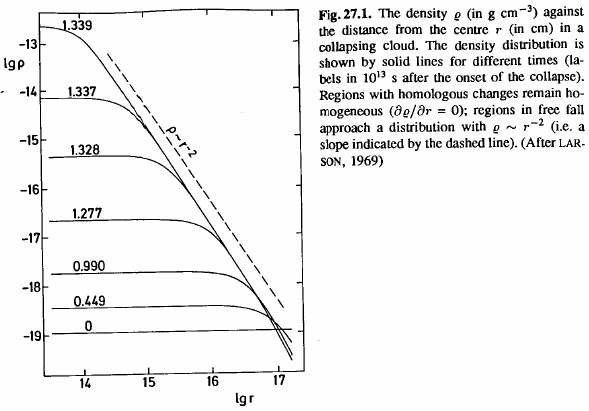
\includegraphics[trim={0cm 0cm 1cm 0cm},clip, keepaspectratio,width=0.8\textwidth]{collapsingdensity}\label{fig:collapsingdensity}
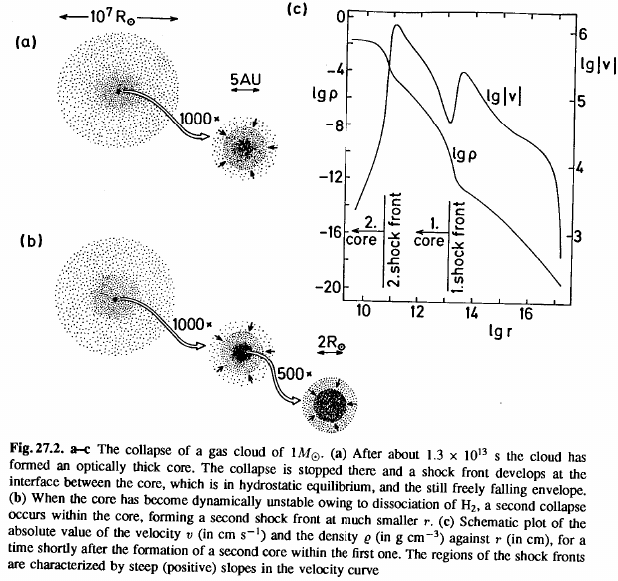
\includegraphics[trim={0cm 0cm 1cm 0cm},clip, keepaspectratio,width=0.8\textwidth]{collapsedensitystructure}\label{fig:collapsedensitystructure}
\end{figure}
\end{column}
\end{columns}
\end{frame}

\begin{frame}{core collapse}
\begin{columns}[T]
	\begin{column}{0.55\textwidth}
	\begin{itemize}
	\item For $H_2$ $\gamma_{ad}=\frac{f+2}{f}=\frac{7}{5}=1.4\approx\frac{4}{3}\approx1.33$, for $H$ $\gamma_{ad}=\frac{5}{3}\approx1.667$.  Slight decreases of $\gamma_{ad}<\frac{4}{3}$ by $H_2$ dissociation: collapse.
	\item When all hydrogen is dissociated $\gamma_{ad}>\frac{4}{3}$
	\item Central compression (of innermost core) is adiabatic as $\tau_{accr}<\tau_{KH}$, then $\dot{M}\to0$ and evolution is no more adiabatic.
	\end{itemize}
	\end{column}
	\begin{column}{0.45\textwidth}
	\begin{figure}[!ht]
	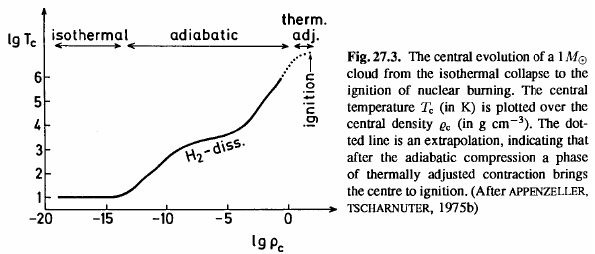
\includegraphics[trim={0cm 0cm 1cm 0cm},clip, keepaspectratio,width=0.99\textwidth]{centralcollapseevolution}\label{fig:centralcollapseevolution}
	\end{figure}
	\end{column}
\end{columns}
\end{frame}

\begin{frame}{Evolution of protostar in HR}
\begin{itemize}
\item Far from HE: radiation emitted by core is absorbed by envelope's grain and re-emitted in IR. Infalling envelope. Start on far right in HR diagram.
\item Thinning of envelope: photosphere moves downward until reaches core - $T_{ff}$ increases
\item In accretion phase $L\approx L_{accr}\propto\dot{M}$, then $L\approx L_g$ of core. Strong accretion rate heats core and make it isothermal, then a T gradient builds up and convection developes downward from surface - we found object on HL if fully convective, normal condition at border and envelope is thin in V.
\end{itemize}
\end{frame}

\subsection{Pre main sequence ed approccio a ZAMS per stelle di sequenza superiori/inferiori}\linkdest{preMS}

\begin{frame}{Traccia di Hayashi}
Primo/secondo core di Larson; Evoluzione di PMS sulla traccia di Hayashi; ruolo di opacit\'a di H- nella verticalit\'a della traccia di Hayashi; fusione deuterio; stelle completamente convettive o con nucleo radiativo. Abbondanza elementi leggeri in stelle di pre-sequenza
\end{frame}


\begin{frame}{Jeans mass ($\num{e5}\msun$)}
\todo{Instability} $\omega^2=k^2c_s^2-4\pi G\rho<0$:
\[\lambda>\lambda_H=\sqrt{\frac{\pi c_s^2}{G\rho}}=\SI{0.19}{\parsec}\sqrt{\frac{T}{\SI{10}{\kelvin}}}(\frac{n_{H^2}}{\SI{e4}{\per\cubic\cm}})\expy{-1/2}\]
\end{frame}

\begin{frame}{Protostar: first core and main accretion}
Virial T. $2E_i+\Omega=0$: $3kT\frac{M}{\mu m_H}=\int_0^M\frac{Gm}{r}\,dm$: collapse $\frac{3kTM}{\mu m_H}<\frac{3}{5}\frac{GM^2}{R}$ - $M>M_J=(\frac{3}{4\pi\rho})\expy{1/2}(\frac{5kT}{G\mu m_H})\expy{3/2}\propto T\expy{\frac{3}{2}}\rho\expy{-\frac{1}{2}}$
$t_{ff}\approx(G\rho)\expy{-\frac{1}{2}}\ll t_{cool}$: collasso adiabatico $P\propto T\expy{5/2}$ ($PT\expy{\frac{\gamma}{1-\gamma}}$) - $t_{ff}\gg t_{cool}$: collasso isotermo - \keyword{fragmentation}: Hydrostatic core surrounded by ff gas ($0.01\msun$) \todo{star formation hydrostatic core}
\end{frame}
